\documentclass[conference]{IEEEtran}
\ifCLASSINFOpdf
\else
\fi
\usepackage{graphicx}
\usepackage{amssymb,amsmath,bm}
\usepackage{textcomp}
\usepackage{verbatim} 
\def\vec#1{\ensuremath{\bm{{#1}}}}
\def\mat#1{\vec{#1}}

\begin{document}

\title{Group Delay Functions for Speaker Diarization}

\author{
\IEEEauthorblockN{{ Mohit Yadav, Anil K Sao, A D Dileep and Padmanabhan Rajan}\\
Indian Institute of Technology Mandi, India\\ 
\  {\small \tt mohit\_yadav@students.iitmandi.ac.in \& \{anil, addileep and padman\}@iitmandi.ac.in}
}
}

\maketitle


\begin{abstract}

Speaker Diarization is the task of determining {\bf\textit{``who spoke when"}}
in a speech recording of an unknown duration containing an unknown number of
speakers. The very unsupervised nature of this task makes it more challenging
and demanding for the used features to be highly discriminative across speakers.
Popularly used spectrum-related features for speaker diarization take into
account merely the magnitude information and do not utilize phase information
due to the complications involved in its processing. However, the information
embed in phase has been shown beneficial for (mostly supervised) speech tasks,
now it is being explored for speaker diarization. In this work, we propose
group-delay functions based features for speaker diarization. Group-delay
functions are the representations of phase of Fourier spectrum, which overcomes
the issues in processing the phase. We present our experiments and results on a
publicly available meeting corpus. Our experiments demonstrate that the features
derived from group-delay functions provide comparable or improved diraization
accuracy over and on fusion with the popularly used mel-frequency cepstrum
coefficients (MFCC) features. \\

\end{abstract}
\IEEEpeerreviewmaketitle

%\noindent{\bf Index Terms}: Speaker diarization, group-delay functions, all-pole model, agglomerative information-bottleneck.


\section{Introduction}
\label{intro}

Developments in processing power has made possible the digitization of
large-volume spoken documents like news broadcasts, meetings, lectures 
\cite{reviewPaper2,reviewPaper3}. With this digitization, the utility of speaker
diarization systems has increased tremendously because of their applicability to a large 
number of speech applications \cite{reviewPaper1,reviewPaper4}. These applications 
include information retrieval, speech and speaker indexing, 
document content structuring, speaker recognition in presence of multiple or
competing speakers and to help in speech-to-text transcription. Two popular
approaches for speaker diarization are based on hidden Markov models-Gaussian
mixture models (HMM-GMM) \cite{reviewPaper1} and on
the information-bottleneck (IB) principle \cite{aIB2}. In this paper, we focus on the IB principle based approach as it presents a non-parametric solution and also has computational advantages over the
other approach \cite{aIB2}.

%\subsection{Related Work}
In recent years, the scientific community has seen significant amount of work on
improving features for diarization systems. Broadly this work can be divided
into three categories: (a) spatial information fusion, (b) 
robust overlapped speech handling and (c) learning-based features. Spatial
information fusion based methods exploit multiple recordings acquired using a microphone array often 
referred as multiple-distance-microphones (MDM) \cite{aIB3,aIB4,featAngle,speakerUPM,featSpatial,MDM}. 
These methods enjoy the resultant spatial redundancy, and claim to provide complementary features to
conventionally used MFCC features \cite{MDM}. On the other hand, the approaches from the other two categories do not make any explicit use of spatial information arising from MDM. However, they do make use of a single enhanced recording obtained after beamforming multiple recordings obtained from MDM \cite{beamforming}.

The next category of methods are motivated by fact that the effective handling of
overlapped speech is considered to be at the limits of the current 
state-of-the-art of speaker diarization systems \cite{reviewPaper1,featOverLap}. In the same
spirit, authors in \cite{featProsody,featOverLap} have explored long-term
conversational and prosodic features to detect and handle overlapped speech more
robustly. Authors in \cite{featSC} have also shown improvements for overlap speech detection and handling 
using features based on a convolutive non-negative sparse-coding approach. 
The last category of approaches advocate the use of features
obtained by applying learning-based methods. Authors in \cite{featANN}, have
proposed an artificial neural network-based based approach to learn a feature transform,
aimed to distinguish segments from different speakers. Similarly, authors in
\cite{featPCAnLDA} utilize traditional principal component analysis (PCA) and
linear discriminant analysis (LDA) to perform feature selection, at the initial
and the final stages of diarization respectively. With an exception to
above mentioned categories, authors in \cite{featFilterBank}, have applied
features derived using filter-bank-slope of the magnitude spectrum, and attributed their success to their ability to emphasize
formants. 

Feature derived from magnitude spectrum such as MFCC are ubiquitously used in various
speech tasks. On the other hand, use of the phase of short-term spectrum is not so
widespread, due to the difficulties in its processing.
However, there has been a significant increase in the interest to utilize
information from the phase spectrum recently
\cite{phaseImportantInterspeech14,gdSurvey}. Traditionally, \textit{group delay functions}
and their variants have been used to mitigate difficulties involved in
processing of the phase. Features derived from
group delay functions have shown promise for other speech tasks, and here we 
explore it for speaker diarization \cite{modifiedGD,allPoleGdSid}. 

In this work, we apply features derived from group delay functions for
IB based speaker diarization. The primary objective
is to investigate whether group delay based features can be used
effectively in the context of speaker diarization and if they can supplement magnitude-based
features. The layout for the remaining paper is as follows: section \ref{fe} introduces
group delay functions and difficulties involved in their
processing. Subsequently, section \ref{system} discusses the used IB-based diarization
system briefly. Next in section \ref{feature_analysis_and_fusion}, we present the performed comparative and fusion analysis on the features derived from group delay functions. Their performance is evaluated 
in context of the introduced diarization system on the used AMI dataset (\cite{AMIData}) in section \ref{experimentsNresults}. Lastly in section \ref{conclude}, we conclude and also provide directions for future work.    

\section{Group delay functions}
\label{fe}
Let us denote a frame of speech as $x(n)$ and its Fourier transform as
$X(\omega)$. The polar representation of $X(\omega)$ can be written as follows:

\begin{equation}
X(\omega) = |X(\omega)| e^{j\theta(\omega)} 
\label{equ:FT}
\end{equation}     
where $|X(\omega)|$ and $\theta(\omega)$ refers to magnitude and phase part of
the spectrum respectively. The group delay function is defined as the
negative derivative of the continuous (i.~e.~unwrapped) phase of Fourier transform, and can be written
as follows: 
\begin{equation}
\tau(\omega) =  - \frac{d}{d\omega} \theta(\omega).
\label{equ:GDF_def}
\end{equation}

The high-resolution and additive properties of group delay functions have been
studied earlier (\cite{yegnaJASA, gdSurvey}). As a result of this, in the
group delay domain, very closely
spaced spectral peaks (or valleys) are confined to narrow regions around poles
(or zeros.) However, computation of unwrapped phase of Fourier transform is a
non-trivial task. To bypass this, the group delay function can be computed
directly from the speech signal, without phase unwrapping, as
\cite{gdDerivationIcassp}:

\begin{equation}
\tau(\omega) = \frac{X_R(\omega)Y_R(\omega) +
X_I(\omega)Y_I(\omega)}{|X(\omega)|^{2}},
\label{eq:GDF_com}
\end{equation}

where $y(n) = n x(n)$, and $Y(\omega)$ is its Fourier transform. 
Subscripts $R$ and $I$ in equation \ref{eq:GDF_com}, represents real and
imaginary part of Fourier transform respectively. 

The proximity of a zero (spectral dip) near the
unit circle results in a very small value of the denominator in
equation \ref{eq:GDF_com}. This results in spikes of large magntide in the group
delay spectrum. As a result, the formant information present in the group delay
spectrum is masked. More details about the behaviour of group delay functions
can be found in \cite{gdSurvey}.

To address the above mentioned issues, the
\textit{modified group delay function} (MODGDF) has been proposed
\cite{modifiedGD}, which can
computed using the following expression:
\begin{equation}
\tau_{m}(\omega) =  
\frac{X_R(\omega)Y_R(\omega) + X_I(\omega)Y_I(\omega)}{|S(\omega)|^2}, 
\label{eq:MODGDF}
\end{equation}
where, $|S(\omega)|$ is obtained from $|X(\omega)|$ by cepstral smoothing.
Features derived from the modified group delay function have been used in
several speech tasks \cite{modifiedGD}.
%And parameters $\alpha:(0,1]$ and
%$\gamma:(0,1]$ are used to control its dynamic range. Again, subscripts $R$ and
%$I$, represent real and imaginary part of Fourier transform respectively. 
Another method to overcome the limitations of equation \ref{eq:GDF_com} is to
derive the group delay function from an all-pole model. Such a parametric
representation of group delay functions was first described in \cite{yegnaJASA}.
The parametric model used is
\begin{equation}
H(\omega) =  \frac{G}{1 - \sum_{k=1}^{k = p} a_k e^{-j\omega k}}.
\label{eq:homega}
\end{equation}
Here, $p$ is the model order, and the gain factor $G$ is set to unity. The
model parameters $a_k$ are estimated by solving the standard Yule-Walker
equations. As the filter contains only poles, the spectrum $H(\omega)$ will not have any zeros.
Computing the group delay function from the phase spectrum of $H(\omega)$ will
not result in spurious peaks, as in equation \ref{eq:GDF_com}. The resulting
filter is minimum-phase, and thus has some information loss when compared to the
signal spectrum $X(\omega)$. Features derived from the all-pole group delay
function have been used earlier for speaker recognition \cite{allPoleGdSid}.

\section{Information-bottleneck based diarization}
\label{system}

%{\{c_1,c_2,..,c_K\}}

The information bottleneck (IB) principle states that input variable $X$ should achieve a compact
clustering representation $C$ (bottleneck) and also try to maximize the
information retained with respect to variable of interest $Y$, i.e., a relevance
variable. Formally, IB criterion can be written as follows:

\begin{equation}
\label{eq:aIB}
F = I(Y,C) - \frac{1}{\beta}I(X,C) 
\end{equation} 

where $\beta$ decides trade off between compactness achieved for data $X$ and
information preserved with respect to $Y$. The mentioned criterion is optimized
with respect to stochastic mapping between $C$ and $X$, i.e., $p(c|x)$ . 

The agglomerative IB based diarization starts with detecting speech/non-speech
frames in a given speech recording \cite{aIB2}. Subsequently, fixed length
(typically for $2.5$ seconds) speech-segments are obtained by performing a
uniform and linear segmentation only on the speech frames detected in previous step. Each of 
these speech-segments are more likely to be generated by one speaker, as the duration
is very small. Collectively, these speech segments are used to define the input
variable $X={\{x_i\}}$. After that a Gaussian mixture model(GMM) with shared
diagonal covariance is learned such that each component of GMM utilizes data
from one speech segment only. Each component of the learned GMM is used as one instance of
relevance variable, i.e., $Y = \{ y_{j}\}$. The above defined $X$ and $Y$ are
then fed into the algorithm to obtain the optimal clustering representation $C$. 

Initially, each speech-segment $x_i \in X$ is a separate cluster, and after that
at each step, two clusters are iteratively merged so that decrease in the above
mentioned IB criterion is minimum \cite{aIB2}. The process is repeated until all
clusters are merged into one cluster finally. The optimal number of clusters
is decided based on empirically determined threshold for Normalized mutual
information(NMI), which is defined as the fraction of information preserved in
clustering representation $C$ about $Y$ out of the total amount of information
contained in $X$ about relevance variables $Y$, i.e., $\frac{I(Y,C)}{I(Y,X)}$.
The value of NMI decreases monotonically with respect to number of the clusters,
and decrease in the NMI value is expected to be higher when more dissimilar clusters
(possibly belonging to different speakers) start merging.  After clustering
speech-segments, the Viterbi realignment based on ergodic HMM is used to refine
the initially created speaker boundaries (for details see \cite{aIB2}).

%\begin{comment}
\begin{figure}[h]
\centering
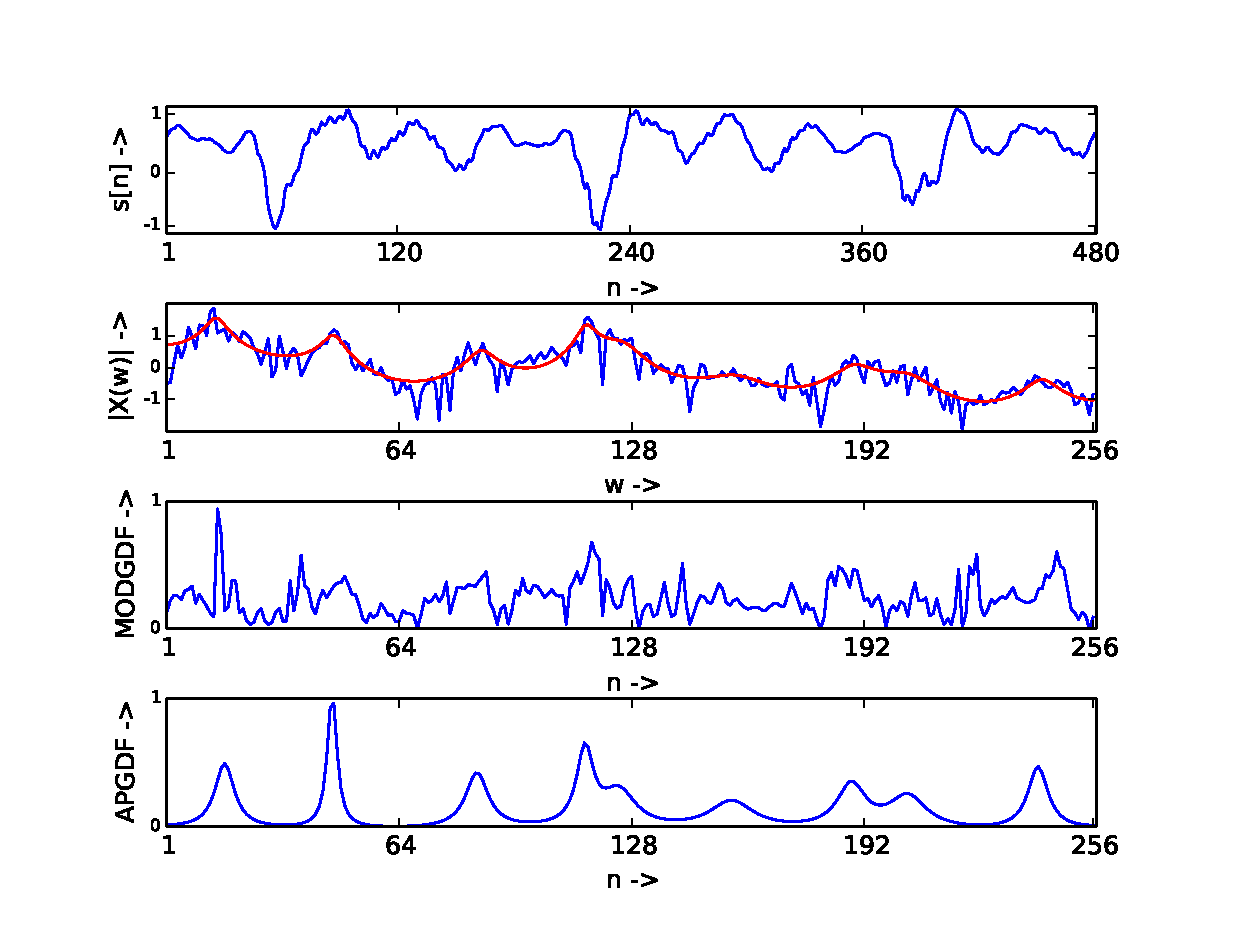
\includegraphics[width=0.5\textwidth,height=10cm]{figures/apSpectrum.eps}
\caption{ A frame of speech (in the top panel), corresponding magnitude of
Fourier spectrum(DFT) and its approximation by all-pole model (in the second
panel), modified group-delay function (in third panel) and all pole model based
group delay function (in the bottom panel).}
\label{fig:all-pole}
\end{figure}
%\end{comment}



\section{Feature Analysis}
\label{feature_analysis_and_fusion}

To show the effectiveness of group-delay based features, we compare and fuse
them with widely know MFCC features as detailed below in Section
\ref{feature_analysis} and Section \ref{feature_fusion} respectively.

\subsection{MFCC v/s Group-delay based features}
\label{feature_analysis}
In order to show the effectiveness of group-delay based features, i.e., MODGDF
and APGDF, we measure Kullback-Leibler (KL) divergence on speech segments, i.e.
$X={x_i}$ created to initiate the aIB clustering algorithm. All choose two
speech segments among all available segments with in a speech recordings, are
divided into inter-speaker and intra-speaker pairs, based on ground-truth of
speakers. We computed mean and variance of KL divergence for both intra-speaker
and inter-speaker pairs, as depicted in Table.\ref{table:kl-div}. For this task,
we select $20$ recordings of different meetings from the entire available AMI
meeting corpus used in our experiments. 


\begin{table}[h]
\centering

\label{table:kl-div}
\begin{tabular}{|l|l|l|}
\hline
Feature 			& Intra-speaker 			& Inter-speaker 	 \\ \hline
MFCC          			& 6.7/10.1               & 8.3/11.4       \\ \hline
MODGDF        			& 6.1/9.7                & 8.4/12.7       \\ \hline
APGDF         			& 5.5/9.7                & 8.6/11.9        \\ \hline
\end{tabular}

\vspace{0.4cm}
\caption{KL divergence for both inter-speaker and intra-speaker speech segments
created at to initialize the aIB clustering algorithm.}
\end{table}

As it is clearly evident from the results in Table \ref{table:kl-div}, the mean
and variance of KL divergence values of intra-speaker and inter-speaker are
decreased and increased for both MODGDF and APGDF respectively. Mean and
variance of KL divergence for intra-speaker has decreased which potentially
indicates the discriminative power of MODGDF and APGDF for speaker information
in the IB framework. Additionally, one must also notice that mean and variance
of KL divergence for inter-speaker has also slightly increased for MODGDF and
APGDF, which further adds on to show their ability to hold speaker information
for IB framework based diarization.  

\subsection{MFCC with Group-delay based features}
\label{feature_fusion}
The IB based diarization system can be easily extended to fuse multiple
features. For each feature stream, we learn a separate GMM with equal number of
components and every component is aligned with speech segment used to initiate
aIB. This enforces unique relationship among the learned GMM for different
feature streams. In other words, if $\lbrace F_1,F_2,...,F_N \rbrace$ are the
features to fuse, where $N$ is the number of features, than corresponding
background model will have components $\lbrace
M^{F_{1}},M^{F_{2}},...,M^{F_{N}}\rbrace$ corresponding to every feature stream.
And the distribution for $p(y|x)$ can be computed as follows:       

\begin{equation}
p(y|x) = \sum _{i=1}^{N} W_i \times p(y|x^{F_{i}},M^{F_{i}})
\label{eq:feat_combs}
\end{equation}

One must notice that features are fused at the level of relevance variables,
which allow to fuse probabilities instead of likelihoods, hence less affected by
the number of dimensions of every feature stream (\cite{aIB}). Unfortunately, it
introduces optimization of $W_i$ parameters, which is an computationally
intensive task as for every new $W_i$ requires further optimization for
parameters present in $p(y|x^{F_{i}},M^{F_{i}})$, e.g, $\beta$ of aIB.

%\begin{comment}
\begin{figure}[h]
\centering
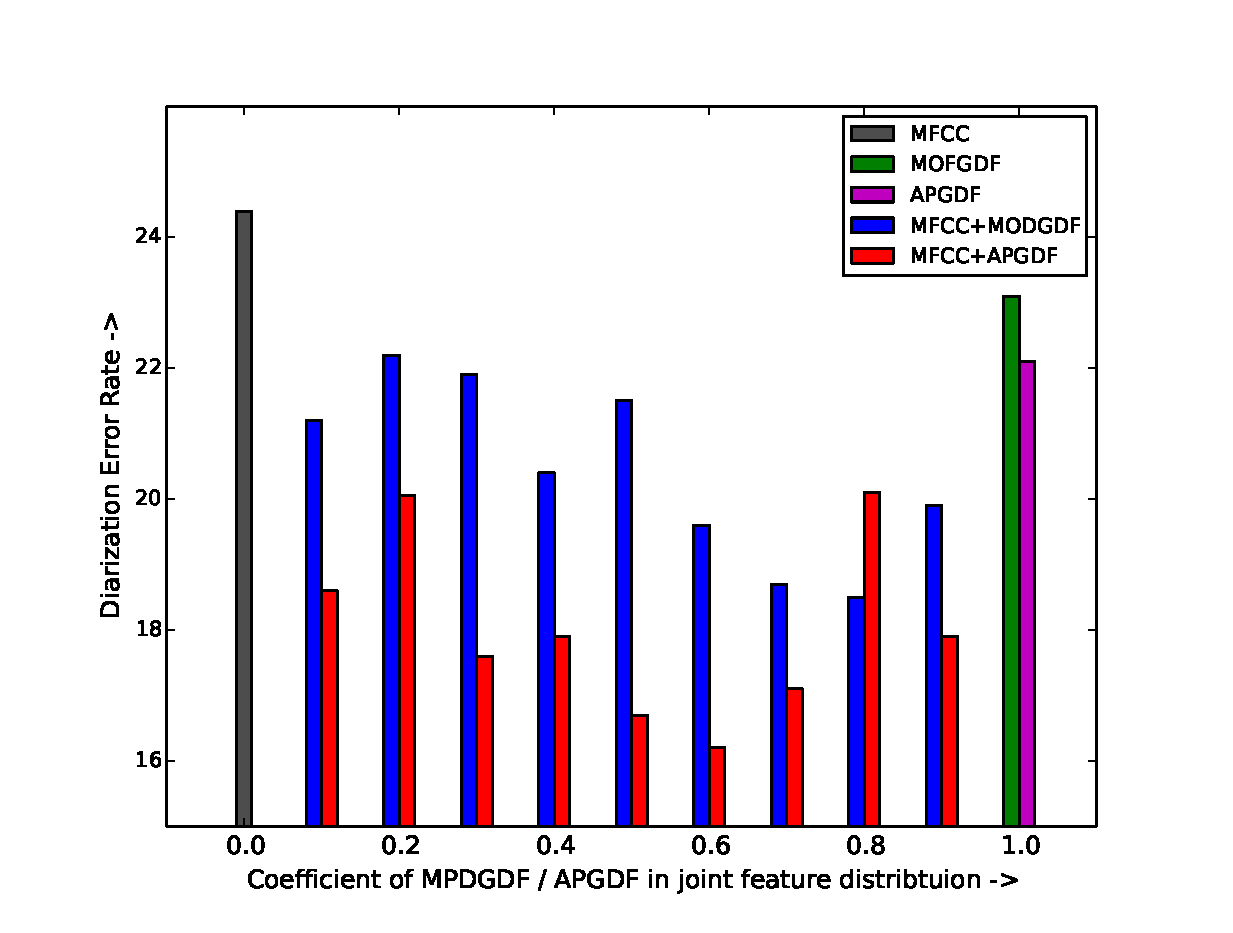
\includegraphics[width=0.5\textwidth,height=5.5cm]{figures/newFusionResults.eps}
\caption{Performance on AMI dataset comparing MFCC and its fusion with MODGDF
and APGDF with respect to weight of probabilities used for MODGDF and APGDF
features. Fusion weights are mentioned in parentheses.}
\label{fig:fusionResults}
\end{figure}
%\end{comment}
Sum of all $W_i$ is bound to be $1$. Fig. \ref{intro} shows improvement in
diarization error with increase in weight ($W_{MODGDF/APGDF}$) of probabilities
arising from distribution of MODGDF and APGDF initially. Beyond a threshold,
further increase in weight ($W_{MODGDF/APGDF}$) results in the deterioration of
the performance as clearly visible in Fig. \ref{fig:fusionResults}.   

\section{Experiments and Results}
\label{experimentsNresults}

We evaluate the performance of the proposed group-delay based features for
speaker diarization on publicly available AMI meeting corpus \cite{AMIData}. In
our experiments, we select 100 meetings out of the total 170 meetings present in
AMI corpus. Data is further divided into two parts, namely, development set
consists of $30$ meetings and test set consists of remaining $70$ meetings.
Optimal values of $\beta$ for aIB clustering and fusion weights (in case of
feature fusion) are selected based on the performance on development set.
Diarization error rate(DER) is used to measure the performance of various
features. The definition of DER is as follows: 
\begin{equation}
DER = MISS + FA + SER
\end{equation}
\begin{comment}
\begin{equation}
	SER = \frac{\sum \limits_{s} {T_s ( min(N_{r}(s),N_{h}(s)) - N_{c}(s) ) } }  { \sum \limits_{s} T_s N_{r}(s)}
\end{equation}
\end{comment}

where MISS, FA and SER represents  missed speech errors, false alarm speech
error, and speaker error (for details on DER see \cite{NIST}). In all the
reported results, we have used the ground-truth speech/non-speech labels to drop
non-speech segments of the meeting, which let DER indicate the speaker
discriminative power more precisely. For optimization of fusion weights, we only
look for $10$ values between $0$ and $1$ as shown in Fig.
\ref{fig:fusionResults}.

\begin{comment}
\begin{figure}[h]
\centering
\includegraphics[width=0.5\textwidth,height=5.5cm]{Images/devNtest.png}
\caption{Fusion results}
\label{fig:fusionResults}
\end{figure}
\end{comment}

\subsection{Feature extraction using MODGDF and APGDF}

We perform frame-blocking with 50\%-overlapping windows of length 30 ms. Number
of filters and length of feature vector for MFCC computation are $40$ and $18$
respectively. The procedure to compute MODGDF can be described below:

\begin{enumerate}
\item Compute discrete Fourier transform for speech frame $X[n]$ and its time
multiplied version $Y[n]=nX[n]$.
\item Perform cepstrally smoothing on $|X(\omega)|$ to estimate $|S(\omega)|$
and plug it into Eg. \ref{eq:MODGDF} to obtain $\tau_{m}(\omega)$.
\end{enumerate}	
\vspace{0.2cm}
Procedure to compute APGDF can be described as follows:
\begin{enumerate}
\item Perform all-pole analysis(LP/WLP) on frame with prediction order set to
$p=20$ and estimate values of coefficients $a(k)$ of all-pole filter.  
\item Use $G=1$ and $a(k)$ to compute frequency response $H(\omega)$ as defined
in Eq. \ref{eq:homega}.
\item Now, group-delay function is computed by taking the negative derivative of
the phase response of $H(\omega)$. Derivative is computed using sample-wise
difference.
\end{enumerate}	
\vspace{0.2cm}
After computing MODGDF and APGDF, we perform discrete cosine transform and keep
the first $18$ coefficients (excluding the zeroth one) in the feature
representation. Additional parameters involved in MODGDF and APGDF ($\alpha =
0.9$, $\gamma=0.4$ and $p=20$) are picked from earlier studies done for speech
and speaker recognition \cite{modifiedGD} and \cite{allPoleGdSid}. We omitting
the search for the optimal value of the additional involved parameters due to
two reasons: 1) As this task is highly computationally intensive
experimentations, and 2) the fact that the primary motivation is to demonstrate
whether group-delay based features are at all capable of improvement in the
diarization systems. Search for optimal values to further refine the results is
left for the future research.

%\begin{comment}
\begin{table}[h]
\centering
\label{my-label}
\begin{tabular}{|l|l|l|}
\hline
Feature Used  & Development Set & Test Set \\ \hline
MFCC          & 24.4                   & 26.3            \\ \hline
MODGDF        & 23.1                   & 25.1            \\ \hline
APGDF         & 22.1                   & 24.9            \\ \hline
MFCC + MODGDF(0.8,0.2) & 18.5          & 20.1            \\ \hline
MFCC + APGDF(0.6,0.4)  & 16.2          & 18.7            \\ \hline
\end{tabular}
\vspace{0.4cm}
\label{table:results}
\caption{Diarization error obtained on AMI dataset comparing various feature
streams and their combinations. In case of fusion, optimum weights are mentioned
in parentheses.}
\end{table}
%\end{comment}


\subsection{Results}

Table \ref{table:results} presents the results of various features and their
combinations used for speaker diarization. Performance of MODGDF and APGDF
fairly indicate that group-delay based features have the ability to represent
speakers for IB based diarization system successfully. The relative improvements
of $4.56\%$ and $4.56\%$ are obtained by MODGDF and APGDF with respect to MFCC
respectively. Fusion of group-delay based features with MFCC has also been
studied and the results of fusion experiments are reported for both MODGDF and
APGDF as MFCC + MODGDF and MFCC + APGDF in Table \ref{table:results}
respectively. The results indicate, as expected, the fusion of MFCC with
group-delay based features have the potential to further push the performance up
of the current diarization systems, as relative improvements of $23.5\%$ and
$28.9\%$ for MFCC + MODGDF and MFCC + APGDF have been observed respectively.

Fusion weights for MFCC + MODGDF and MFCC + APGDF are found (0.8,0.2) and
(0.6,0.2) respectively. We suspect relatively lesser improvements provided by
MODGDF when compared to APGDF are due to omitted search process for parameters
involved in its computation. Results show that performance of diarization system
start improving on increase of the probability arising from the individually
learned distribution of group-delay based features, as it is clearly evident
from the Fig. \ref{fig:fusionResults}. Interestingly, we found there is always
an improvement for any choice of fusion weight, when compared to both MFCC and
group-delay based features standalone.     


\section{Conclusion And Future Work}
\label{conclude}
In this work, we investigated the use of group-delay based features in IB based
diarization system. Using with and without model based techniques, namely,
MODGDF and APGDF, to estimate group-delay function and used them further to
derive features for diarization. We found that features derived from MODGDF and
APGDF provide better diarization error rate. Furthermore, fusion with MFCC has
yielded a significant improvement in the diarization accuracy.  In future, it
will be particularly interesting to further investigate their performance in
more complex scenarios, e.g., for overlapped speech and speech/non-speech
detection at early stage of a diarization system. Additionally, fusion study of
other spectral and time domain features with group-delay based features appears
reasonable direction to explore further. 

\bibliographystyle{IEEEbib}
\bibliography{bare_conf}

\end{document}


